\section{Implementación}

Respecto a la implementación, el software para balancear las clases está implementado en Python mientras que los algoritmos utilizados están implementados en C++.

Como sistema de control de versiones se ha utilizado el software Git, y el código se encuentra alojado y liberado en GitHub \cite{githubProyecto}, bajo una licencia GNU GPLv3 \cite{gplv3}.

Todo el código está documentado utilizando Doxygen \cite{doxygen}, de forma que es posible acceder a la documentación de todas las clases, métodos, funciones y definiciones del código.

\subsection{Preprocesado}

De cara al preprocesado simplemente se han implementado funciones que reciben como entrada los datos y realizan las correspondientes transformaciones, así como funciones para realizar un conteo de clases. También se ha desarrollado un script en Python que será el encargado de realizar el sobremuestreo de datos para las clases minoritarias, como se comento en la sección del preprocesado de datos.

\subsection{Algoritmos}

Con respecto a la implementación de los algoritmos utilizados, estos se han implementado en C++.

La implementación tiene un enfoque orientado a objetos, además de ciertas funciones auxiliares que utilizaremos a lo largo de la implementación. De cara a implementar las distintas clases necesarias así como las funciones se ha encapsulado todo en un espacio de nombres de C++ que se llamará \texttt{algoritmos\_poblacion\_expresiones}. Esto nos evitará problemas de definiciones si en un futuro se utiliza el software para otros proyectos, además de dar una mejor estructura del código.

\subsubsection{Clase AlgoritmoPoblacion}

El código esta estructurado utilizando herencia y plantillas de C++, de forma que nos encontramos con una clase \texttt{AlgoritmoPoblacion<T>}, que tiene como plantilla la clase de expresión que utilizará dicho algoritmo. Esta clase será abstracta, y nunca se podrá utilizar por si misma.

Esta clase contendrá los datos y métodos comunes a cualquier algoritmo que utilice una población, de forma que las operaciones comunes estén definidas y no sea necesario repetir código si necesitamos hacer distintas variaciones. De cara a implementar un algoritmo simplemente se ha de crear una clase que derive de esta e implemente un método \texttt{ajustar}, que será el que se encargue de ajustar dicho algoritmo concreto, además de todo lo que se considere oportuno.

\begin{figure}[H]
	 \centering
	 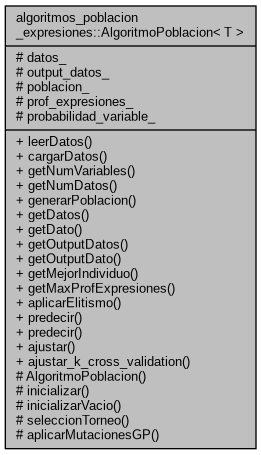
\includegraphics[width=0.2\textwidth]{clases/algoritmo_poblacion.png}
	 \caption{Diagrama de la clase AlgoritmoPoblacion.}
	\label{fig:diagrama_clase_algoritmo_poblacion}
\end{figure}


\subsubsection{Clase Poblacion}

La clase \texttt{AlgoritmoPoblacion<T>} contiene una población, la cual será un conjunto de datos de tipo \texttt{T}, que puede realizar ciertas operaciones concretas, en este caso encapsularemos dichas operaciones y atributos en la clase \texttt{Poblacion<T>}.

Estas clase se tratará de una clase de consulta de cara a almacenar todos los individuos que entran en juego en nuestros algoritmos, así como una forma de aplicar ciertas operaciones a todos los individuos, como por ejemplo evaluarlos.

\begin{figure}[H]
	 \centering
	 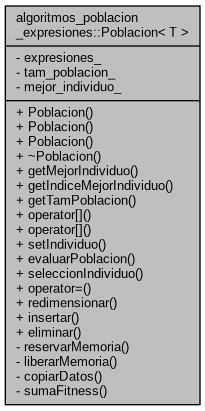
\includegraphics[width=0.2\textwidth]{clases/poblacion.png}
	 \caption{Diagrama de la clase Poblacion.}
	\label{fig:diagrama_clase_poblacion}
\end{figure}

\newpage

\subsubsection{Clase Expresion}

Una vez tenemos la parte genérica de un algoritmo con una población de expresiones, necesitamos una estructura que nos represente dichas expresiones, en este caso, la clase \texttt{Expresion}. Esta clase será la expresión original de Programación Genética, que contendrá un árbol que conformará la expresión. Este árbol se ha representado como un vector con la representación en preorder del árbol.

En esta clase encontraremos como atributos el propio árbol, el ajuste de dicha expresión, la longitud máxima que permitiremos que tenga la expresión, entre otros atributos auxiliares. También podemos encontrar como métodos distintas operaciones de las expresiones de Programación Genética, como intercambiar un subárbol, evaluar la expresión con ciertos datos, entre otras.


\begin{figure}[H]
	 \centering
	 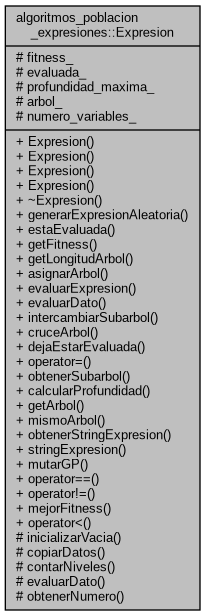
\includegraphics[width=0.2\textwidth]{clases/expresion.png}
	 \caption{Diagrama de la clase Expresion.}
	\label{fig:diagrama_clase_expresion}
\end{figure}

\subsubsection{Clase Nodo}

Dichos árboles de las expresiones serán un conjunto de nodos, el cual representaremos con la clase \texttt{Nodo}. Cada nodo podrá ser de un tipo distinto y nosotros utilizaremos los siguientes tipos:

\begin{itemize}
	\item Variable: Indica que el nodo se refiere a una variable del conjunto de datos de entrada.
	\item Número: El nodo será una constante numérica.
	\item Más: Operador de suma.
	\item Menos: Operador de resta.
	\item Por: Operador de multiplicación.
	\item Entre: Operador de división.
\end{itemize}

Hemos escogido pocos operadores de cara a mantener las expresiones resultantes simples.

\begin{figure}[H]
	 \centering
	 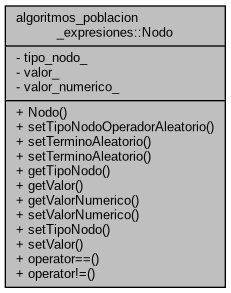
\includegraphics[width=0.2\textwidth]{clases/nodo.png}
	 \caption{Diagrama de la clase Nodo.}
	\label{fig:diagrama_clase_nodo}
\end{figure}

\newpage

\subsubsection{Clase AlgoritmoPG}

Esta clase se trata de la clase del algoritmo de Programación Genética que implementamos. Esta clase \texttt{AlgoritmoPG} será una clase hija de \texttt{AlgoritmoPoblacion<Expresion>}, es decir, el algoritmo de Programación Genética es un algoritmo con una población de \texttt{Expresion}.

\texttt{AlgoritmoPG} simplemente implementa el método \texttt{ajustar}, que será la forma en la que el algoritmo se ajuste para los datos y etiquetas dados.


\begin{figure}[H]
	 \centering
	 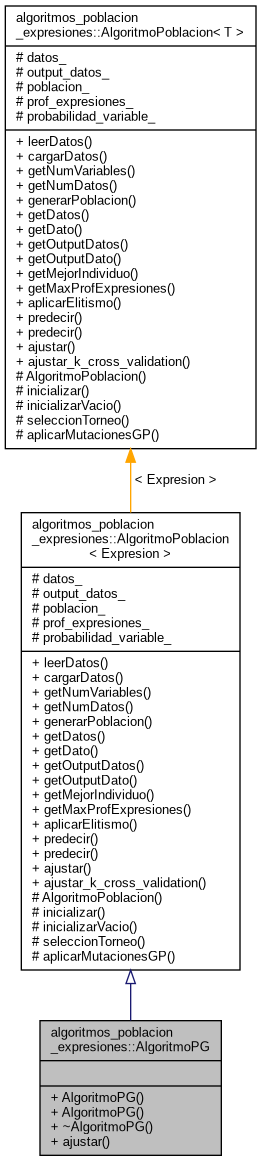
\includegraphics[width=0.2\textwidth]{clases/algoritmoPG.png}
	 \caption{Diagrama de la clase AlgoritmoPG.}
	\label{fig:diagrama_clase_algoritmoPG}
\end{figure}

\newpage

\subsubsection{Clase Expresion\_GAP y AlgoritmoGAP}

Como vemos, con la estructura de clases con plantillas introducir un nuevo algoritmo es tan simple como definir el comportamiento de la expresión a utilizar y como se ajusta dicho algoritmo a los datos. Por este motivo, introducir la variante de GA-P es muy simple.

Para las expresiones de GA-P usaremos como base las expresiones de Programación Genética, ya que el único añadido es el cromosoma, los operadores de cruce y mutación de GA-P y la forma en la que se obtienen los valores numéricos, por lo tanto la clase \texttt{Expresion\_GAP} quedará de la siguiente forma.



\begin{figure}[H]
    \centering
	 \begin{subfigure}[b]{0.49\textwidth}
		 \centering
		 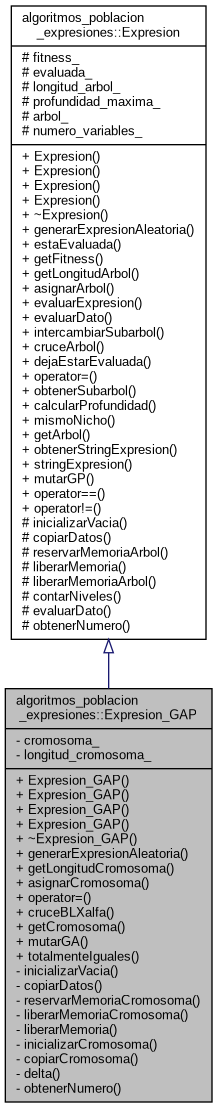
\includegraphics[width=0.3\textwidth]{clases/expresion_gap.png}
		 \caption{Diagrama de la clase Expresion\_GAP.}
		\label{fig:diagrama_clase_expresion_gap}
	 \end{subfigure}
	\begin{subfigure}[b]{0.49\textwidth}
		 \centering
		 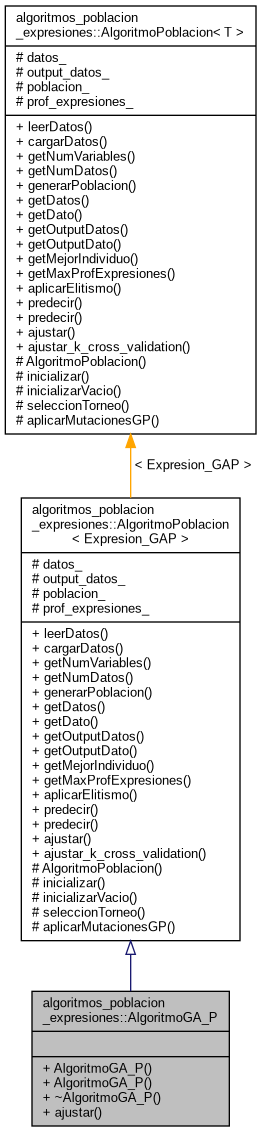
\includegraphics[width=0.3\textwidth]{clases/algoritmo_gap.png}
 		\caption{Diagrama de la clase Algoritmo\_GAP.}
 	  \label{fig:diagrama_clase_algoritmo_gap}
   \end{subfigure}

	\caption{Diagrama de clases de Algoritmo\_GAP y Expresion\_GAP.}
	\label{fig:diagrama_clases_gap}
\end{figure}


\subsubsection{Clase Parametros}

De cara a hacer más sencillo el uso de los algoritmos también se ha implementado una clase \texttt{Parametros} que contiene todos los parámetros posibles para los algoritmos. De esta forma gestionar los parámetros con los que se lanza un algoritmo es mucho más sencillo, además de que nos permite una mayor flexibilidad a la hora de realizar distintas ejecuciones.

\begin{figure}[H]
	 \centering
	 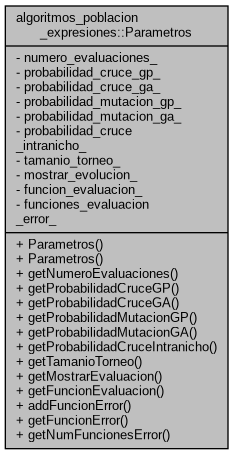
\includegraphics[width=0.2\textwidth]{clases/parametros.png}
	 \caption{Diagrama de la clase AlgoritmoPG.}
	\label{fig:diagrama_clase_parametros}
\end{figure}


\subsubsection{Diagrama de clases final}

Con todas estas clases, el diagrama final quedaría de la siguiente forma:

\begin{figure}[H]
	 \centering
	 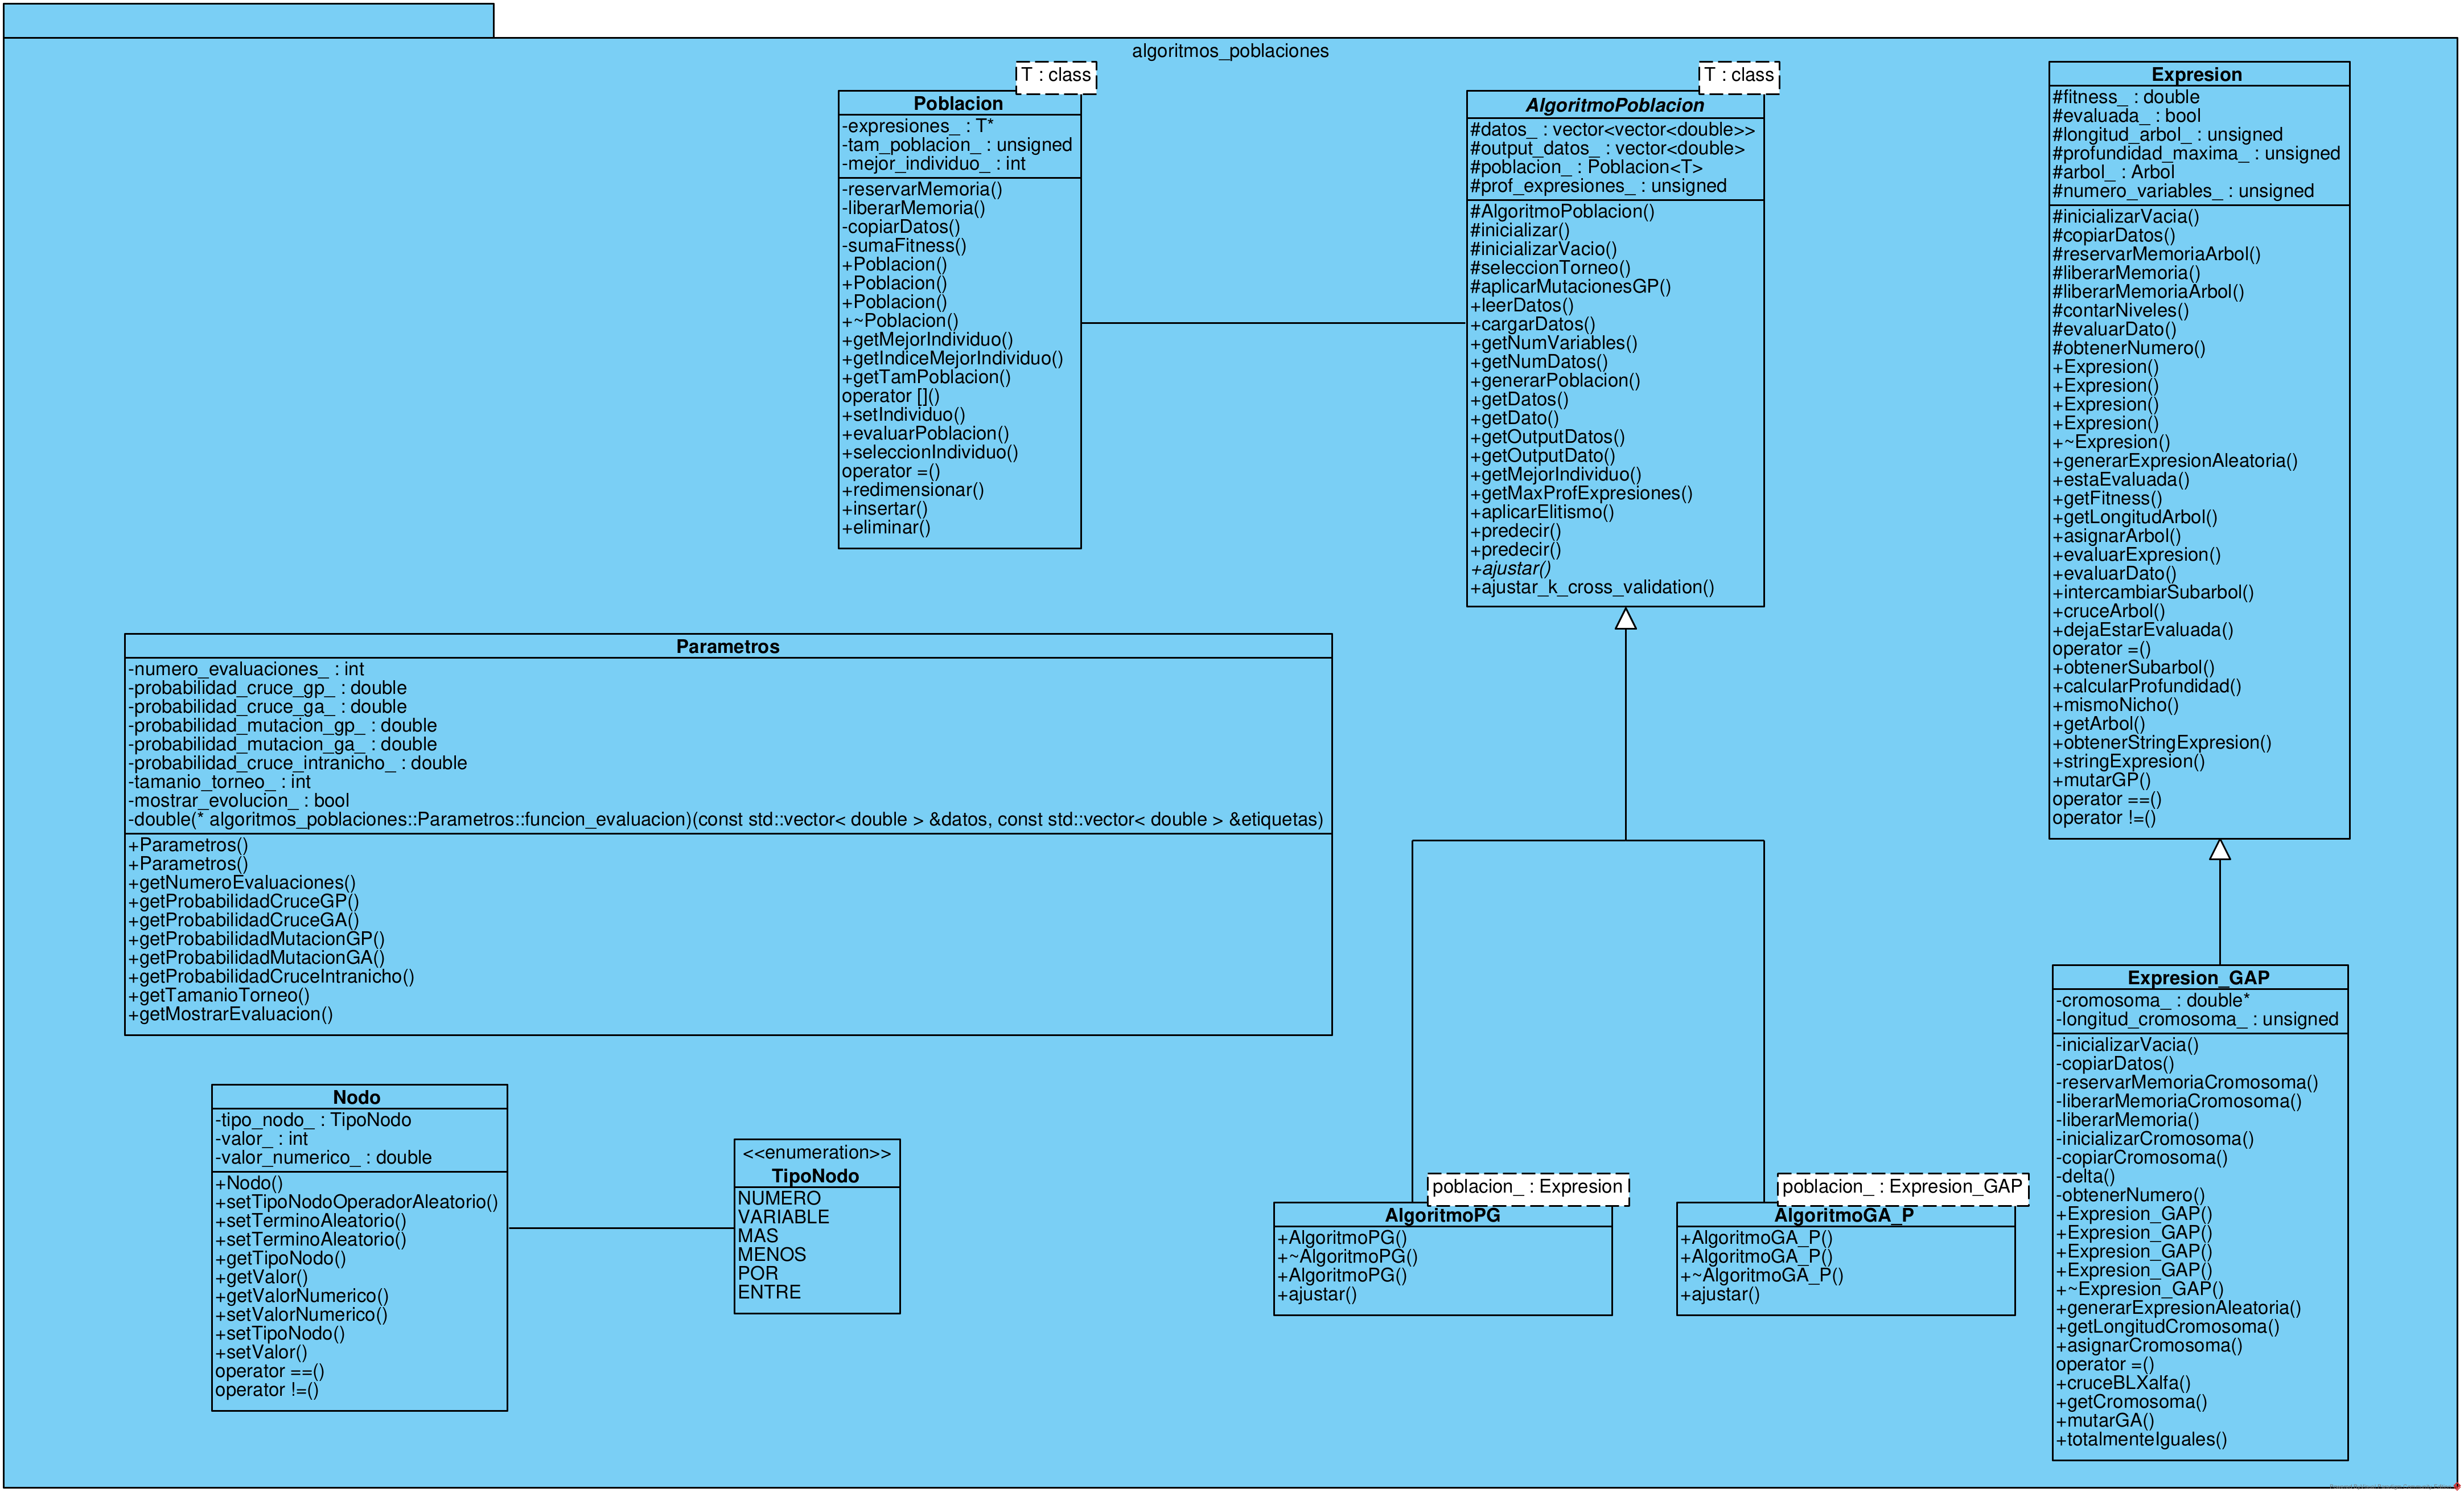
\includegraphics[width=\textwidth]{clases/diagrama_clases.png}
	 \caption{Diagrama de clases.}
	\label{fig:diagrama_clases}
\end{figure}

Cabe destacar algunas declaraciones de tipos internas que se han hecho, como la del tipo \texttt{funcion\_evaluacion\_t}, que se trata de un puntero a una función que recibe una matriz de datos y un vector de etiquetas y devuelve un real. Esta función será la función que utilicemos para evaluar las expresiones, pero debido a su complejidad sintáctica se ha definido este tipo para que nombrarlo sea más fácil. El tipo completo sería:

\begin{lstlisting}[language=C++]
double (*funcion_evaluacion_t)(const std::vector<double> & datos, const std::vector<double> & etiquetas)
\end{lstlisting}

\subsubsection{Otras funciones auxiliares}

También disponemos de algunas funciones auxiliares, que nos servirán a lo largo de todo el código, como la comprobación de si dos valores reales son iguales teniendo en cuenta los problemas de representación de números en coma flotante de C++, o distintas posibles funciones de evaluación que hemos predefinido.

\newpage

\subsection{Validación de los algoritmos}


Uno de los problemas que nos encontramos en los algoritmos de aprendizaje automático es la validación del algoritmo, es decir, como podemos asegurar que nuestro algoritmo realmente funciona, y no se trata de que ha hecho un sobreajuste con los datos con los que ha entrenado y fuera de dichos datos no es capaz de realizar buenas predicciones.

Para comprobar y asegurarnos que los algoritmos son capaces de realizar buenas predicciones fuera de los datos con los que ha entrenado utilizaremos validación cruzada con $k$ iteraciones.

Este método consiste en dividir el conjunto de entrenamiento en $k$ partes de mismo tamaño, de forma que realizaremos $k$ iteraciones para entrenar nuestro modelo. En cada iteración utilizaremos una de estas partes como conjunto de validación y las otras $k - 1$ partes como conjunto de entrenamiento, de forma que el algoritmo no haya entrenado con esa parte de validación. Finalmente para obtener el error del algoritmo para dicho conjunto de datos utilizaremos la media del error en los distintos conjuntos de validación de cada iteración.

Es importante destacar que antes de hacer las separaciones en $k$ subconjuntos de datos el conjunto de entrenamiento se reordenará de forma aleatoria para evitar que un conjunto en el que los datos estén ordenados por clase se excluya del entrenamiento cierta clase, porque todas sus muestras están en el conjunto de validación.

De esta forma podremos obtener un valor del error del algoritmo para unos datos con los que no ha entrenado, a la vez que comprobamos que nuestro algoritmo es capaz de ajustarse bien o no a un conjunto de datos.


\begin{figure}[H]
    \centering

	 \begin{subfigure}[b]{\textwidth}
		\centering
		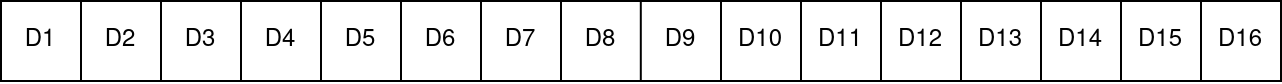
\includegraphics[width=0.8\textwidth]{cross_validation/conjunto_datos.png}
		\caption{Ejemplo de un conjunto de 16 datos.}
	  \label{fig:ej_16_datos}
   \end{subfigure}
	\vspace{1cm}

	 \begin{subfigure}[b]{\textwidth}
		 \centering
		 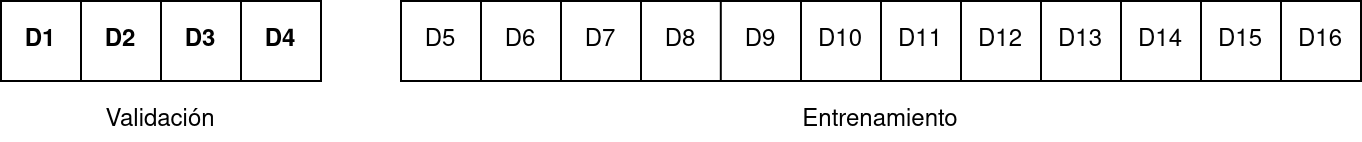
\includegraphics[width=0.8\textwidth]{cross_validation/iteracion1.png}
 		 \caption{Separación entre validación y entrenamiento en la primera iteración.}
 	    \label{fig:cv_iteracion1}
	 \end{subfigure}
	 \vspace{1cm}

	\begin{subfigure}[b]{\textwidth}
		 \centering
		 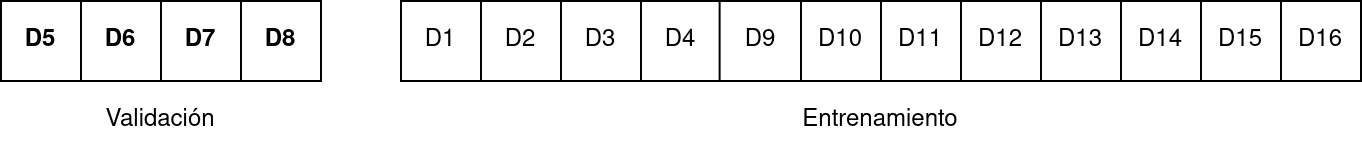
\includegraphics[width=0.8\textwidth]{cross_validation/iteracion2.png}
 		 \caption{Separación entre validación y entrenamiento en la segunda iteración.}
 	    \label{fig:cv_iteracion2}
   \end{subfigure}
	\vspace{1cm}

	\begin{subfigure}[b]{\textwidth}
		 \centering
		 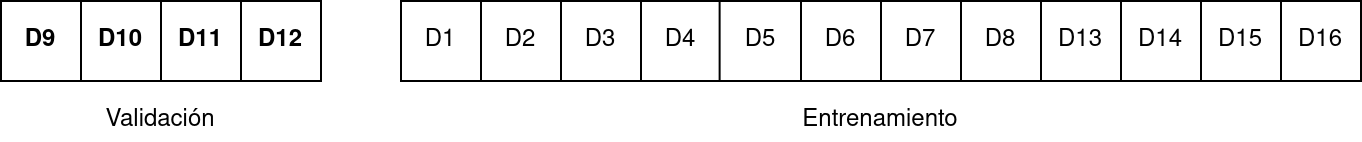
\includegraphics[width=0.8\textwidth]{cross_validation/iteracion3.png}
 		 \caption{Separación entre validación y entrenamiento en la tercera iteración.}
 	    \label{fig:cv_iteracion3}
	\end{subfigure}
	\vspace{1cm}

	\begin{subfigure}[b]{\textwidth}
		 \centering
		 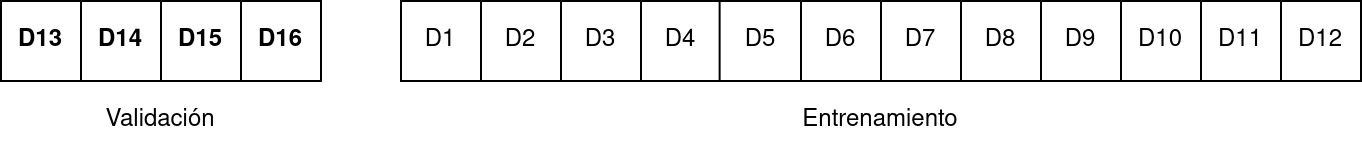
\includegraphics[width=0.8\textwidth]{cross_validation/iteracion4.png}
 		 \caption{Separación entre validación y entrenamiento en la cuarta iteración.}
 	    \label{fig:cv_iteracion4}
	\end{subfigure}

	\caption{Ejemplo de validación cruzada de 4 iteraciones.}
	\label{fig:4-cv-ejemplo}
\end{figure}


\subsubsection{Validación cruzada utilizando 5x2cv}

En nuestro caso utilizaremos 5x2cv para validación. Este método fue propuesto por Thomas G. Dietterich en el año 1998 \cite{propuesta5x2cv}.

Este método se basa en realizar cinco repeticiones de una validación cruzada con dos iteraciones, cada una de estas repeticiones utilizando particiones distintas de los datos al 50\%. De esta forma, con cada una de las cinco particiones que realicemos a los datos aplicaremos una validación cruzada con dos folds, entrenando con la primera mitad de los datos y validando con la segunda mitad en el primer fold, y al contrario en el segundo fold.

Como podemos ver, con cinco repeticiones y siendo cada una de estas un 2-cv (de ahí el nombre 5x2cv) obtendremos diez valores de error, siendo el error final obtenido en validación la media de estos diez valores.



\newpage

\subsection{Funciones de evaluación}

De cara a evaluar los algoritmos necesitaremos una función de evaluación que nos permita saber el error que estamos cometiendo en las estimaciones.

En nuestro caso, al realizar una regresión simbólica, utilizaremos tres medidas:

\begin{itemize}
	\item Error cuadrático medio.
	\item Raíz del error cuadrático medio.
	\item Error absoluto medio.
\end{itemize}

\subsubsection{Error cuadrático medio}

El error cuadrático medio es un estimador que medirá el promedio de los errores cometidos al cuadrado. Esta función de error se utiliza especialmente al entrenar modelos, ya que es muy sensible a errores, lo que ayuda a la hora del aprendizaje a distinguir dos soluciones, aunque el error que cometan ambas sea similar, esta función penalizará mucho más a la que tenga un mayor error.

\begin{figure}[H]
	 \centering
	 $$ ECM = \frac{1}{n} \sum_{i = 1}^{n}(\hat{Y_i} - Y_i)^2 $$
	 \caption{Fórmula para calcular el error cuadrático medio, donde $\hat{Y_i}$ son las etiquetas predecidas y $Y_i$ son las etiquetas reales.}
	\label{fig:ECM}
\end{figure}

\subsubsection{Raíz del error cuadrático medio}

La raíz del error cuadrático medio se trata de aplicar la raíz cuadrada al error cuadrático medio. Este error, al tener la misma escala que las etiquetas reales se utiliza para interpretar directamente el resultado sobre los datos disponibles.

\begin{figure}[H]
	 \centering
	 $$ RECM = \sqrt{ECM} $$
	 \caption{Fórmula para calcular la raíz del error cuadrático medio.}
	\label{fig:RECM}
\end{figure}

\newpage

\subsubsection{Error absoluto medio}

El error absoluto medio (MAE por sus siglas en inglés) se trata de medir la diferencia entre dos valores, en nuestro caso los valores obtenidos y los valores esperados.

\begin{figure}[H]
	 \centering
	 $$ MAE = \frac{\sum_{i = 1}^{n}|\hat{Y_i} - Y_i|}{n} $$
	 \caption{Fórmula para calcular el error absoluto medio, donde $\hat{Y_i}$ son las etiquetas predecidas y $Y_i$ son las etiquetas reales.}
	\label{fig:MAE}
\end{figure}

Con el error absoluto medio podremos observar el error de precisión del modelo al estimar valores, así como comparar con el estado del arte del problema, ya que como vimos, en la mayoría de trabajos se utilizaba esta técnica para medir el error.

\newpage

\subsection{Documentación del proyecto}

Todo el proyecto se ha documentado con Doxygen, y se puede acceder a la documentación a través del fichero \texttt{index.html} de la carpeta \texttt{doc/html} en el código.

En este documento se puede encontrar la estructura del proyecto, así como las distintas opciones de compilación.

\begin{figure}[H]
	 \centering
	 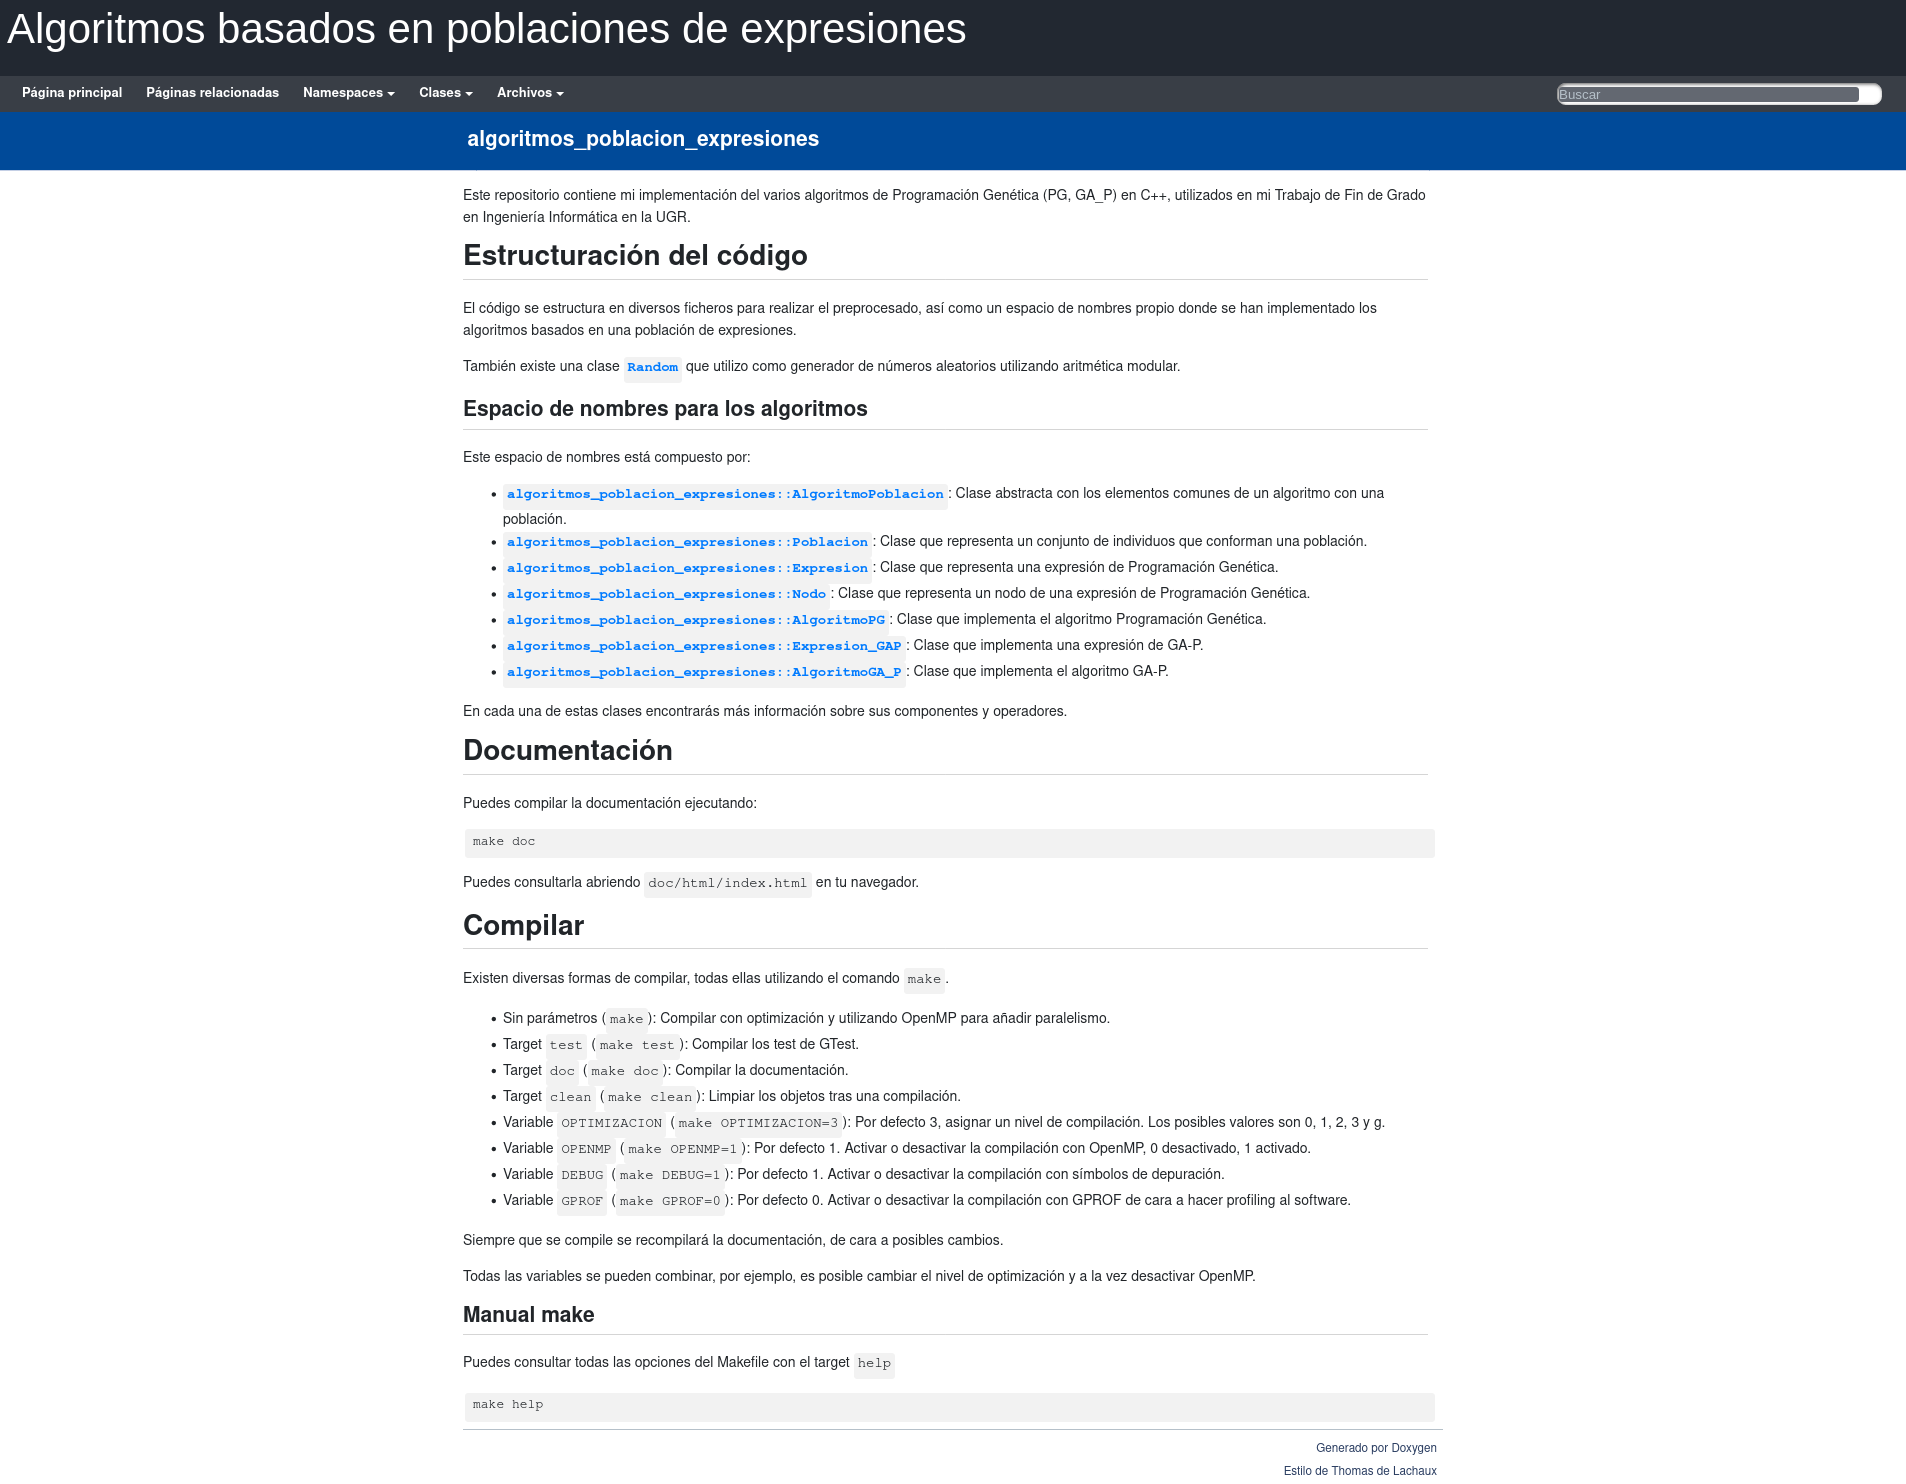
\includegraphics[width=\textwidth]{documentacion.png}
	 \caption{Página principal de la documentación del proyecto.}
	\label{fig:documentación}
\end{figure}

\newpage

\subsection{Verificación del software desarrollado}

De cara a verificar que las distintas clases y métodos desarrollados funcionan utilizaremos GoogleTest \cite{gtest}.

GoogleTest es un entorno de trabajo para verificar software a través de test unitarios.

Los test unitarios son test que evalúan una sección concreta de un software, con el objetivo de comprobar que dicha sección de código funciona de forma correcta, y de esta forma aislar las secciones de código que no se comportan como esperábamos, facilitando la tarea de prueba y corrección de errores en un código.

Para que estos tests nos sean útiles tienen que cumplir las siguientes condiciones:

\begin{enumerate}
	\item Tienen que ser independientes y repetibles. El resultado de un test no debe depender de otros test, de forma que si un test falla este falle por la sección de código que estamos probando, no porque existe un test que no se comporta como creíamos.
	\item Tienen que estar estructurados, y reflejar como funciona todo el conjunto del software. De esta forma es sencillo separar como funcionan las distintas partes del software, permitiendo centrarnos en comprobar que cada parte funciona de forma correcta.
	\item Deben de ser portables y reutilizables. Los tests deben finalizar correctamente independientemente del sistema y compilador utilizado.
	\item Cuando un test falla debe proporcionar tanta información como le sea posible.
	\item Los test han de ser rápidos. El objetivo es comprobar que el software funciona como queremos de una forma rápida, sin perder más tiempo en ejecutar los tests que en compilar y ejecutar el sistema.
\end{enumerate}

Siguiendo estas premisas, se han diseñado tests para cada una de las clases y el conjunto del sistema software. Dichos tests están disponibles en la carpeta \texttt{test} del software, y además el fichero para generar el software ejecutará dichos tests, de forma que si estos tests no son completados correctamente detendrá la compilación.

\newpage

\subsection{Como utilizar y compilar el software}

Existen diversas formas de compilar, todas ellas utilizando el comando `make`.

\begin{itemize}
	\item Sin parámetros (\texttt{make}): Compilar con optimización y utilizando OpenMP para añadir paralelismo.
	\item Target \texttt{test} (\texttt{make test}): Compilar los test de GTest.
	\item Target \texttt{doc} (\texttt{make doc}): Compilar la documentación.
	\item Target \texttt{clean} (\texttt{make clean}): Limpiar los objetos tras una compilación.
	\item Variable \texttt{OPTIMIZACION} (\texttt{make OPTIMIZACION=3}): Por defecto 3, asignar un nivel de compilación. Los posibles valores son 0, 1, 2, 3 y g.
	\item Variable \texttt{OPENMP} (\texttt{make OPENMP=1}): Por defecto 1. Activar o desactivar la compilación con OpenMP, 0 desactivado, 1 activado.
	\item Variable \texttt{DEBUG} (\texttt{make DEBUG=0}): Por defecto 0. Activar o desactivar la compilación con símbolos de depuración.
	\item Variable \texttt{GPROF} (\texttt{make GPROF=0}): Por defecto 0. Activar o desactivar la compilación con GPROF de cara a hacer profiling al software.

\end{itemize}

Siempre que se compile se recompilará la documentación, de cara a posibles cambios.

Todas las variables se pueden combinar, por ejemplo, es posible cambiar el nivel de optimización y a la vez desactivar OpenMP.

Los binarios se generarán en la carpeta \texttt{bin} y cada uno de ellos tiene instrucciones de como utilizarlos.

\newpage

\subsection{Ejecución con un conjunto de datos de prueba}

De cara a probar que nuestra implementación funciona vamos a utilizar un conjunto de datos sencillo, con pocos datos y cuyo funcionamiento es muy simple, Iris \cite{irisDataset}. Este dataset contiene tres características de tres variantes de la flor Iris: Setosa, Versicolour y Virginica. Existen 50 muestras de cada clase, siendo 150 muestras en total.

En principio este problema es de clasificación, pero para hacer esta prueba se han asignado valores numéricos a cada clase, de forma que a cada clase asignaremos un valor numérico, 0, 1 y 2. De esta forma, nuestro algoritmo utilizará las tres características numéricas para predecir el valor numérico que será la clase.


Para la prueba se ha separado el conjunto de entrada en un 80\% de entrenamiento y un 20\% de test. Tras esto se han ajustado los algoritmos usando como validación 5x2cv y los siguientes parámetros:

\begin{itemize}
	\item Tamaño de población: $1.000$.
	\item Probabilidad de que un nodo sea una variable: $30\%$.
	\item Tamaño máximo del árbol: $10$.
	\item Número de evaluaciones: $100.000$.
	\item Probabilidad de cruce en PG: $75\%$.
	\item Probabilidad de cruce en GA: $75\%$.
	\item Probabilidad de mutación en PG: $5\%$.
	\item Probabilidad de mutación en GA: $5\%$.
	\item Probabilidad de cruce intra-nicho: $3\%$.
	\item Tamaño del torneo: $30$.
\end{itemize}

Tras realizar las ejecuciones, obtenemos los siguientes resultados en Programación Genética:

\begin{lstlisting}
RMSE (Root Mean Square Error) en validacion cruzada de: 0.2616322184
\end{lstlisting}

Con las siguientes predicciones sobre el conjunto de test:

\begin{figure}[H]
	 \centering
	 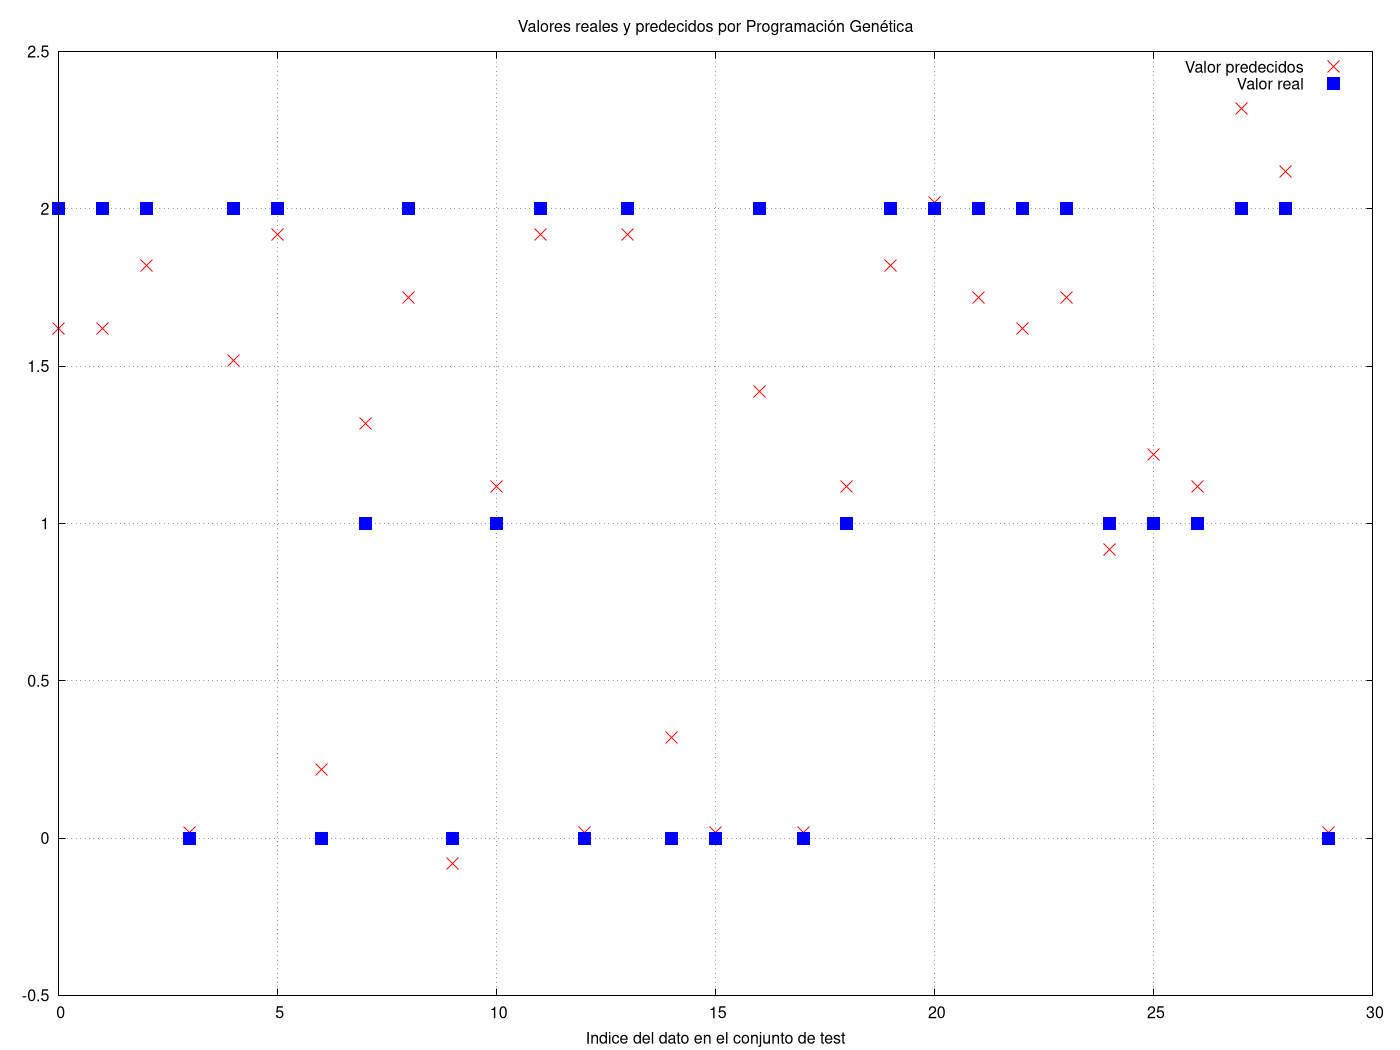
\includegraphics[width=0.8\textwidth]{iris_gp.png}
	 \caption{Comparación de valores reales y predicciones con Programación genetica.}
	\label{fig:iris_gp}
\end{figure}

Y con la siguiente fórmula:

\begin{figure}[H]
	 \centering
	 $$( ( -1.136984  / ( -3.640915  +  9.897730 ) ) +  x3 )$$
	 \caption{Fórmula obtenida de la regresión simbólica con Programación Genética.}
	\label{fig:formula_iris_gp}
\end{figure}

Mientras que en GA-P obtenemos:

\begin{lstlisting}
RMSE (Root Mean Square Error) en validacion cruzada de: 0.24989117
\end{lstlisting}

Con las siguientes predicciones sobre el conjunto de test:

\begin{figure}[H]
	 \centering
	 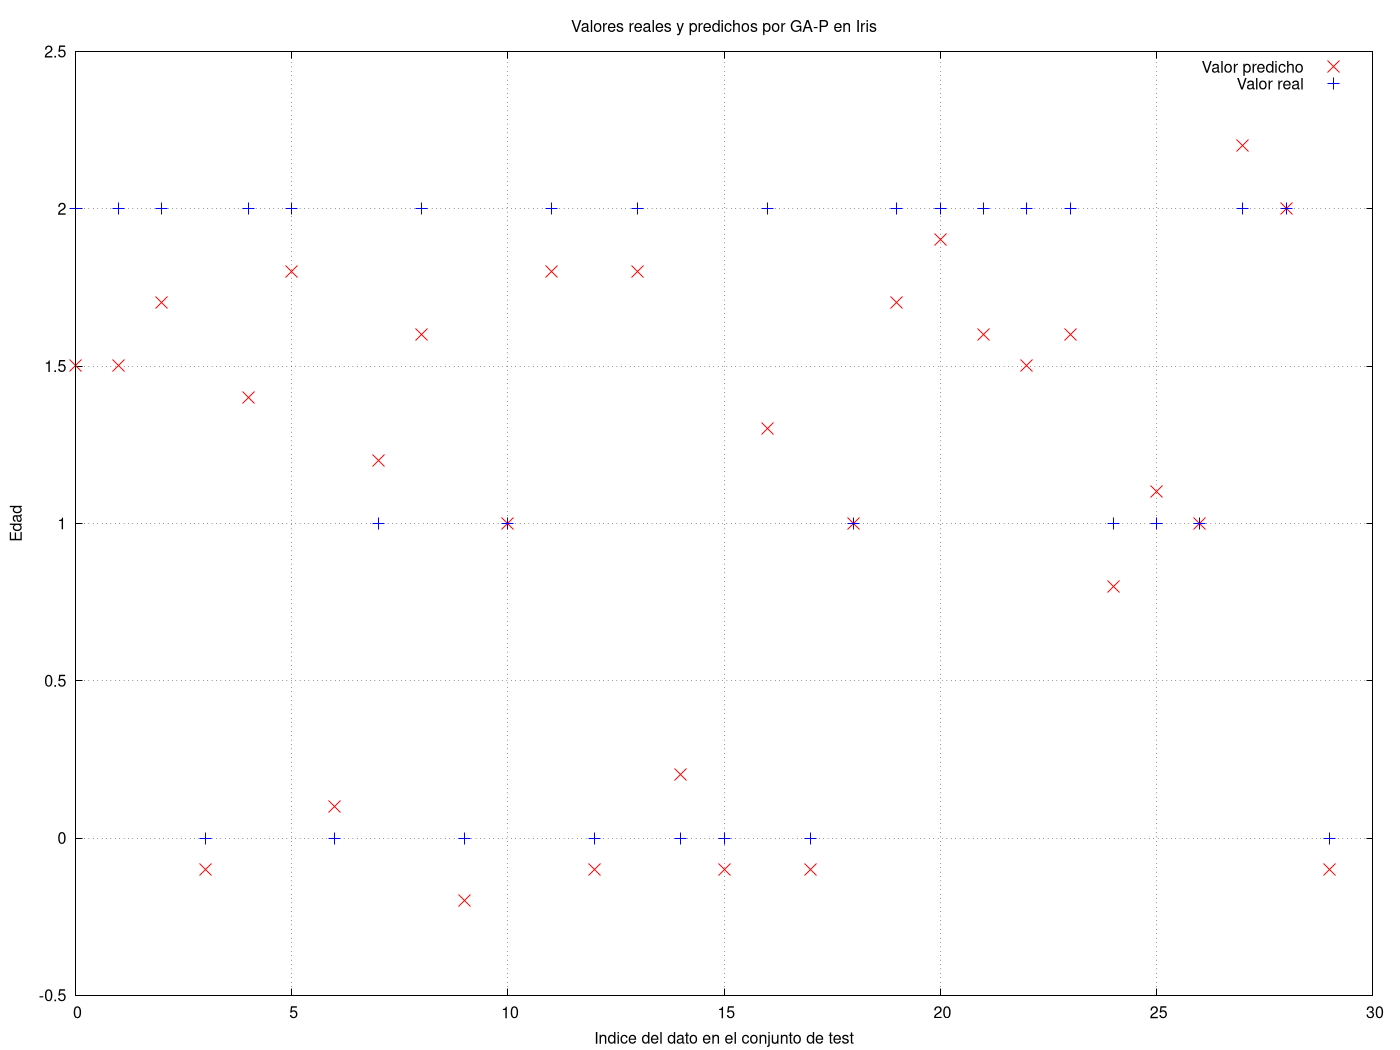
\includegraphics[width=0.8\textwidth]{iris_gap.png}
	 \caption{Comparación de valores reales y predicciones con GA-P.}
	\label{fig:iris_gap}
\end{figure}

Y con la siguiente fórmula:

\begin{figure}[H]
	 \centering
	 $$( -0.299342  +  x_3 )$$
	 \caption{Fórmula obtenida de la regresión simbólica con GA-P.}
	\label{fig:formula_iris_gap}
\end{figure}

Como vemos, el resultado es muy similar, y es que si nos fijamos en las fórmulas obtenidas de la regresión simbólica (figuras \ref{fig:formula_iris_gp} y \ref{fig:formula_iris_gap}), ambas son prácticamente la misma, pero GA-P ha sido capaz de aprender mejor los valores numéricos constantes necesarios y por lo tanto obtener un resultado más compacto, tal y como esperábamos.

\newpage

\subsection{Uso de paralelismo}

Una de las tareas más costosas que nos podemos encontrar en ambos algoritmos es evaluar la población cuando esta tiene un gran número de individuos y el número de datos es muy elevado.

Para reducir el tiempo utilizado por estas tareas podemos aprovechar el paralelismo de los datos. Evaluar una expresión es totalmente independiente de evaluar otra, de forma que esta tarea se puede realizar en paralelo y así reducir el tiempo de ejecución.

También se ha probado el paralelizar la generación de la nueva población en cada generación del algoritmo, ya que en las operaciones de cruce y mutación son independientes entre sí al seleccionar a priori que elementos formarán parte del cruce y mutación, sin embargo esto no ha dado buenos resultados ya que el coste de crear y eliminar los hilos que se ejecutarán en paralelo, sumado a las esperas en secciones críticas esto hacía que el tiempo de ejecución fuera igual o superior a ejecutarlo en secuencial.

\newpage
